%%%%%%%%%%%%%%%%%%%%%%%%%%%%%%%%%%%%%%%%%%%%%%%%%%%%%%%%%%%%%%%%%%%%%%%%%%%%%%%%
\documentclass[twocolumn]{revtex4}

%%%%%%%%%%%%%%%%%%%%%%%%%%%%%%%%%%%%%%%%%%%%%%%%%%%%%%%%%%%%%%%%%%%%%%%%%%%%%%%%
% Note that comments begin with a "%" and are not turned into text in the .pdf
% document.
%%%%%%%%%%%%%%%%%%%%%%%%%%%%%%%%%%%%%%%%%%%%%%%%%%%%%%%%%%%%%%%%%%%%%%%%%%%%%%%%

%%%%%%%%%%%%%%%%%%%%%%%%%%%%%%%%%%%%%%%%%%%%%%%%%%%%%%%%%%%%%%%%%%%%%%%%%%%%%%%%
% Include some extra packages.
%%%%%%%%%%%%%%%%%%%%%%%%%%%%%%%%%%%%%%%%%%%%%%%%%%%%%%%%%%%%%%%%%%%%%%%%%%%%%%%%
\usepackage[]{graphicx}
%%%%%%%%%%%%%%%%%%%%%%%%%%%%%%%%%%%%%%%%%%%%%%%%%%%%%%%%%%%%%%%%%%%%%%%%%%%%%%%%

%%%%%%%%%%%%%%%%%%%%%%%%%%%%%%%%%%%%%%%%%%%%%%%%%%%%%%%%%%%%%%%%%%%%%%%%%%%%%%%%
\begin{document}

%%%%%%%%%%%%%%%%%%%%%%%%%%%%%%%%%%%%%%%%%%%%%%%%%%%%%%%%%%%%%%%%%%%%%%%%%%%%%%%%
\title{
Weather Predictions (Rainfall)
}

\author{Zainab Raza}

\affiliation{Siena College, Loudonville, NY}

\date{\today}

\begin{abstract}
 
This project was about predicting the rainfall using Monte Carlo methods and analytically figuring out probabilities. We had to figure out probabilities of it raining one day out of the month, and then eight days out of the month. I did the problems analytically first so I knew what answer to be expected. After using loops and conditionals, I found out that the percentage of it raining one and only one day out of the month (when the percentage of rain on any given day is 20 percent), would be around 0.92 percent. On the other hand, the percentage of it raining on at least eight days of the month (when the percentage of rain on any given day is 10 percent), no matter the order, would be around 0.77 percent. In order to make the predictions more accurate, I needed to test it with many days/months. 
\end{abstract}

%\vspace{1in}

\maketitle
%%%%%%%%%%%%%%%%%%%%%%%%%%%%%%%%%%%%%%%%%%%%%%%%%%%%%%%%%%%%%%%%%%%%%%%%%%%%%%%%

%%%%%%%%%%%%%%%%%%%%%%%%%%%%%%%%%%%%%%%%%%%%%%%%%%%%%%%%%%%%%%%%%%%%%%%%%%%%%%%%%%%%%%%%%%%%%%%%%%%%%%%%%%%%%%%%%%%%%%%%%%%%%%%%%%%%%%%%%%%%%%%%%
\section{Introduction}
%%%%%%%%%%%%%%%%%%%%%%%%%%%%%%%%%%%%%%%%%%%%%%%%%%%%%%%%%%%%%%%%%%%%%%%%%%%%%%%%
This project on rainfall predictions brought together the concepts of weather and the Monte Carlo concept. The Monte Carlo method provides you with random possibilities and outcomes for decision making. This is used in multiple occupations because of it's power. It's used in finance, engineering, physics, etc. Monte Carlo methods are computational algorithms and rely on randomly testing numbers repeatedly. They are mainly used in probability distribution, optimization, and numerical integration. In this case, we used them for probability. In finance, for example, it can be used to model possible changes in asset prices. The goal was to predict the weather (rainfall) using the Monte Carlo method in Python. We had to figure out the odds that it rains a certain amount of days in a month. We had to do this analytically first with pen and paper. Doing this gave me a estimate of what my number should be around. After that, we had to try to do the same thing numerically in Python using the Monte Carlo method. The Monte Carlo method provides you with random possibilities and outcomes for decision making. A simple example of the Monte Carlo example is with dice. You can test the probability of certain sides with it. No one is actually going to roll the dice a thousand times to check probabilites, but Monte Carlo can. 


\begin{figure}
\centering
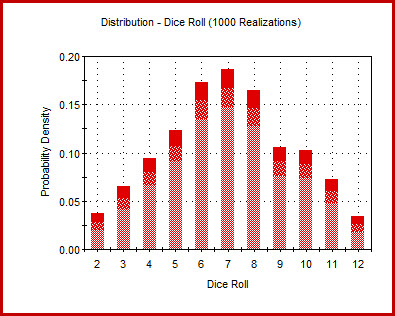
\includegraphics[width=0.3\textwidth]{DiceRoll1000.jpg} 
\end{figure}

As you can see in this figure, through Monte Carlo methods, you are able to see the probability of the sides of dice. It makes life a lot easier when you are dealing with probability and repetition with random numbers. 

%%%%%%%%%%%%%%%%%%%%%%%%%%%%%%%%%%%%%%%%%%%%%%%%%%%%%%%%%%%%%%%%%%%%%%%%%%%%%%%%
\section{Problem 1}
%%%%%%%%%%%%%%%%%%%%%%%%%%%%%%%%%%%%%%%%%%%%%%%%%%%%%%%%%%%%%%%%%%%%%%%%%%%%%%%%
The first problem is about calculating the percent chance of it raining one and only one day out of the month. In this example, there is a 20 percent chance of raining on any given day. As I said above, I did this problem analytically first. Because there is a a 20 percent chance that it will rain on \textit{one day}, I started with 0.2. 1 minus 0.20 is 0.80, and that was the chance that it wouldn't rain. Because it only wanted one day, I know that there was 29 days where it would not rain. For that reason, I did 0.8 to the 29th power. Because there are 30 days in a month in the problem, I multiplied the whole equation by 30. When I did this out, I got 0.00928. This would be 0.9 percent.
$$ (0.2*0.8^{29})^{30} = 0.00928$$
 Now that I knew what the percentage the answer should be around using the Monte Carlo mehtod, this was easier for me. After importing what I needed to in Python (numpy and random), I defined a function. I decided to call my function rainfall. It is important to write out that there are 30 days in a month, so I set a variable equal to 30. I also needed to keep track of the days where it actually rained, so I set a variable equal to zero as a placeholder. After doing that, I did a loop. The range in this loop was zero to the days in a month. I generated a random number anywhere between zero and one. Next, I did conditionals. I wanted to deal with the days that it actually rained first. I did this so that if the random number happened to be between 0 and 0.2, then it would rain. I used a Boolean for this so it would be "True" if it rained. Then, if it did come out true, I set it so that one day would be added for each day that it rained. So what if it doesn't rain? I had to add that if the random number came out to be between 0.20 or 1.0, then there would be no rainfall, so it would be "False." I then tested this by setting the number of days to something much larger than 30 for accuracy. Again, I had to keep track of every day that it rained, so I set a variable to zero.  I then looped over the amount of days that I set and if that was equal to one because you only want one day of rainfall, then you would add another day.  
%%%%%%%%%%%%%%%%%%%%%%%%%%%%%%%%%%%%%%%%%%%%%%%%%%%%%%%%%%%%%%%%%%%%%%%%%%%%%%%%
\section{Problem 2}
%%%%%%%%%%%%%%%%%%%%%%%%%%%%%%%%%%%%%%%%%%%%%%%%%%%%%%%%%%%%%%%%%%%%%%%%%%%%%%%%
The second problem is almost identical to the first one. The only differences are that I need to calculate the percent chance of it raining not one day, but eight days in the month, and the chance of rain is 10 percent on any given day. Once again, I defined a function and set the amount of days in a month as zero, and the placeholder as zero. I also set a variable to generate random numbers from zero to one. This time, I had to set the random variable to be greater than or equal to zero, but less than 0.10. This is because there is only a ten percent chance of rain. I then set that to be "True", and if it was true, then I added a day to the total number of days that it rained. If the random number was not between 0.0 and 0.10, then there would be no rainfall. This means that it would be "False." Once again, I set the amount of days to something greater than 30 and the total number of days that it rained, to zero. In the previous problem, I needed the rainfall to equal one exactly, because there is only one day that it rains. For this question, it is asking for the chance for at least eight days, so I set it so the function would have to be greater than or equal to zero. This gave me the chance that it rains at least eight days in the month to be about 0.7370 percent. 



\end{document}
%%%%%%%%%%%%%%%
